\section{Question 2}
	Refer to the MATLAB code in Appendix 9.a which was used to generate the homogeneous transformation matrices required.\\

	\begin{figure}[position = here]
		\begin{centering}
		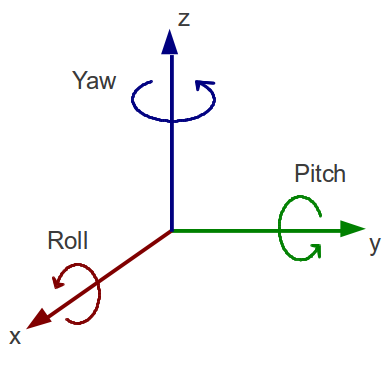
\includegraphics{q2Axes}
		\caption[\textit{RPYAxes}]{Roll Pitch and Yaw definitions (relative to axis names)}
		\end{centering}
	\end{figure}
	
	\subsection{Validity Check}
	We need to prove that the determinant of the matrix is equal to 1 and that the inverse of the matrix is equal to the transpose to prove validity.
		\subsubsection{$R_{1}$}
			$$
			R_{1} =
			\begin{pmatrix}
				0.7500 & -0.4330 & -0.5000\\
				0.2165 & 0.8750 & -0.4330\\
				0.6250  & 0.2165  & 0.7500
			\end{pmatrix}
			$$
			\hspace{35mm}$det(R_{1}) = 1.0000$
			\\
			$$
			R_{1}^{-1} =
			\begin{pmatrix}
				0.7500 & 0.2165 & 0.6250\\
				-0.4330 & 0.8750 & 0.2165\\
				-0.5000  & -0.4330  & 0.7500
			\end{pmatrix}
			$$
			
			$$
			R_{1}^{T} =
			\begin{pmatrix}
				0.7500 & 0.2165 & 0.6250\\
				-0.4330 & 0.8750 & 0.2165\\
				-0.5000  & -0.4330  & 0.7500
			\end{pmatrix}
			$$
			
			\hspace{30mm}$R_{1}^{-1} = R_{1}^{T}\therefore R_{1}$ is \emph{valid}
			
		\pagebreak
		\subsubsection{$R_{2}$}
			$$
			R_{2} =
			\begin{pmatrix}
				0.7725 & -0.4460 & -0.5150\\
				0.2165 & 0.8750 & -0.4330\\
				0.6000  & 0.2078  & 0.7200
			\end{pmatrix}
			$$
			\hspace{35mm}$det(R_{2}) = 0.9888$
			\\
			$$
			R_{2}^{-1} =
			\begin{pmatrix}
				0.7281 & 0.2165 & 0.6510\\
				-0.4204 & 0.8750 & 0.2255\\
				-0.4885  & -0.4330  & 0.7813
			\end{pmatrix}
			$$
					
			$$
			R_{2}^{T} =
			\begin{pmatrix}
				0.7725 & 0.2165 & 0.6000\\
				-0.4460 & 0.8750 & 0.2078\\
				-0.5150  & -0.4330  & 0.7200
			\end{pmatrix}
			$$
			
			$R_{2}^{-1} \approxeq R_{2}^{T}\therefore R_{2}$ is \emph{valid} within the limits of practical numerical applications.
			
		\subsubsection{$R_{3}$}
			$$
			R_{3} =
			\begin{pmatrix}
				0 & 0 & 1\\
				0.8660 & 0.5000 & 0\\
				-0.5000  & 0.8660  & 0
			\end{pmatrix}
			$$
			\hspace{35mm}$det(R_{3}) = 1$
			\\
			$$
			R_{3}^{-1} =
			\begin{pmatrix}
				0 & 0.8660 & -0.5000\\
				0 & 0.5000 & 0.8660\\
				1  & 0  & 0
			\end{pmatrix}
			$$
		
			$$
			R_{3}^{T} =
			\begin{pmatrix}
				0 & 0.8660 & -0.5000\\
				0 & 0.5000 & 0.8660\\
				1  & 0  & 0
			\end{pmatrix}
			$$
		
			\hspace{30mm}$R_{3}^{-1} = R_{3}^{T}\therefore R_{3}$ is \emph{valid}
				
		\subsubsection{$R_{4}$}
			$$
			R_{4} =
			\begin{pmatrix}
				-0.7500 & -0.2165 & -0.6250\\
				0.4330 & -0.8750 & -0.2165\\
				0.5000  & 0.4330  & -0.7500
			\end{pmatrix}
			$$
			\hspace{35mm}$det(R_{4}) = -1$
			\\
			$$
			R_{4}^{-1} =
			\begin{pmatrix}
				-0.7500 & 0.4330 & 0.5000\\
				-0.2165 & -0.8750 & 0.4330\\
				-0.6250  & -0.2165  & -0.7500
			\end{pmatrix}
			$$
				
			$$
			R_{4}^{T} =
			\begin{pmatrix}
				-0.7500 & 0.4330 & 0.5000\\
				-0.2165 & -0.8750 & 0.4330\\
				-0.6250  & -0.2165  & -0.7500
			\end{pmatrix}
			$$
					
			\hspace{30mm}Although $R_{4}^{-1} = R_{4}^{T}, det(R_{4}) \neq 1 \therefore R_{4}$ is \emph{invalid}
					
	\newpage
	\subsection{Roll/Pitch/Yaw Angles}
		Roll Angle is $\alpha$,
		Pitch Angle is $\beta$,
		Yaw Angle is $\gamma$.\\
	Assumption: The believability of the angles can be determined purely mathematically. In reality these angles may not necessarily be believable depending on the application at hand. However, we cannot account for this without further information about the system.
		\subsubsection{$R_{1}$}
		The following values are believable\\
			$\alpha_{1}$ = 16.1021\degree\\ 
			$\beta_{1}$ = -36.6822\degree\\ 
			$\gamma_{1}$ = 16.1016\degree\\
		\subsubsection{$R_{2}$}
		The following values are believable\\
			$\alpha_{2}$ = 15.0665\degree\\
			$\beta_{2}$ = -36.8699\degree\\
			$\gamma_{2}$ = 15.0552\degree\\
		\subsubsection{$R_{3}$}
		The following values are believable\\
			$\alpha_{3}$ = 90\degree\\
			$\beta_{3}$ = 30\degree\\
			$\gamma_{3}$ = 89.5611\degree\\
		\subsubsection{$R_{4}$}
		The following values are not believable as $R_{4}$ is an invalid rotational matrix\\
			$\alpha_{4}$ = 150\degree\\
			$\beta_{4}$ = -30\degree\\
			$\gamma_{4}$ = 29.9990\degree\\
	\subsection{Angle Estimation}
	For a matrix such as $R_{2}$ we can adjust our matrix values slightly (making them less accurate i.e. to fewer decimal values) to still get a reasonable estimation of our angles. We can realise this by seeing that the determinant is so close to 1.
	$R_{4}$, however, cannot give us a reasonable estimate for the angles as the determinant is too far from the required value of 1.
%%	for __ these estimated values would be more realistic